\subsection{Other Information}

%if needed write here other details about your Data Logic Layer that cannot be expressed directly through the ER schema

\subsubsection{Restructuration}
We have decided to restructure the ER scheme deleting the entities TYPE\_ACTION (with relation IS\_OF) and the relation HAS\_ROLES. The modifications made are: \\
\begin{itemize}
    \item HAS\_ROLES has been deleted because we have decided to retrieve the attribute number\_of\_roles using a query.\\
    \item TYPE\_ACTION has been removed and substituted with an attribute type\_action (type: VARCHAR(20)). The field of the attribute is managed with an enumeration.
\end{itemize}
We have decided to improve the efficiency of the app reducing the size of the database. In order to achieve this goal these modifications were necessary.\\
The restructured ER scheme can be seen in the image below [\ref{fig:res_er_scheme}].


\begin{figure}[htbp] 
    \centering
    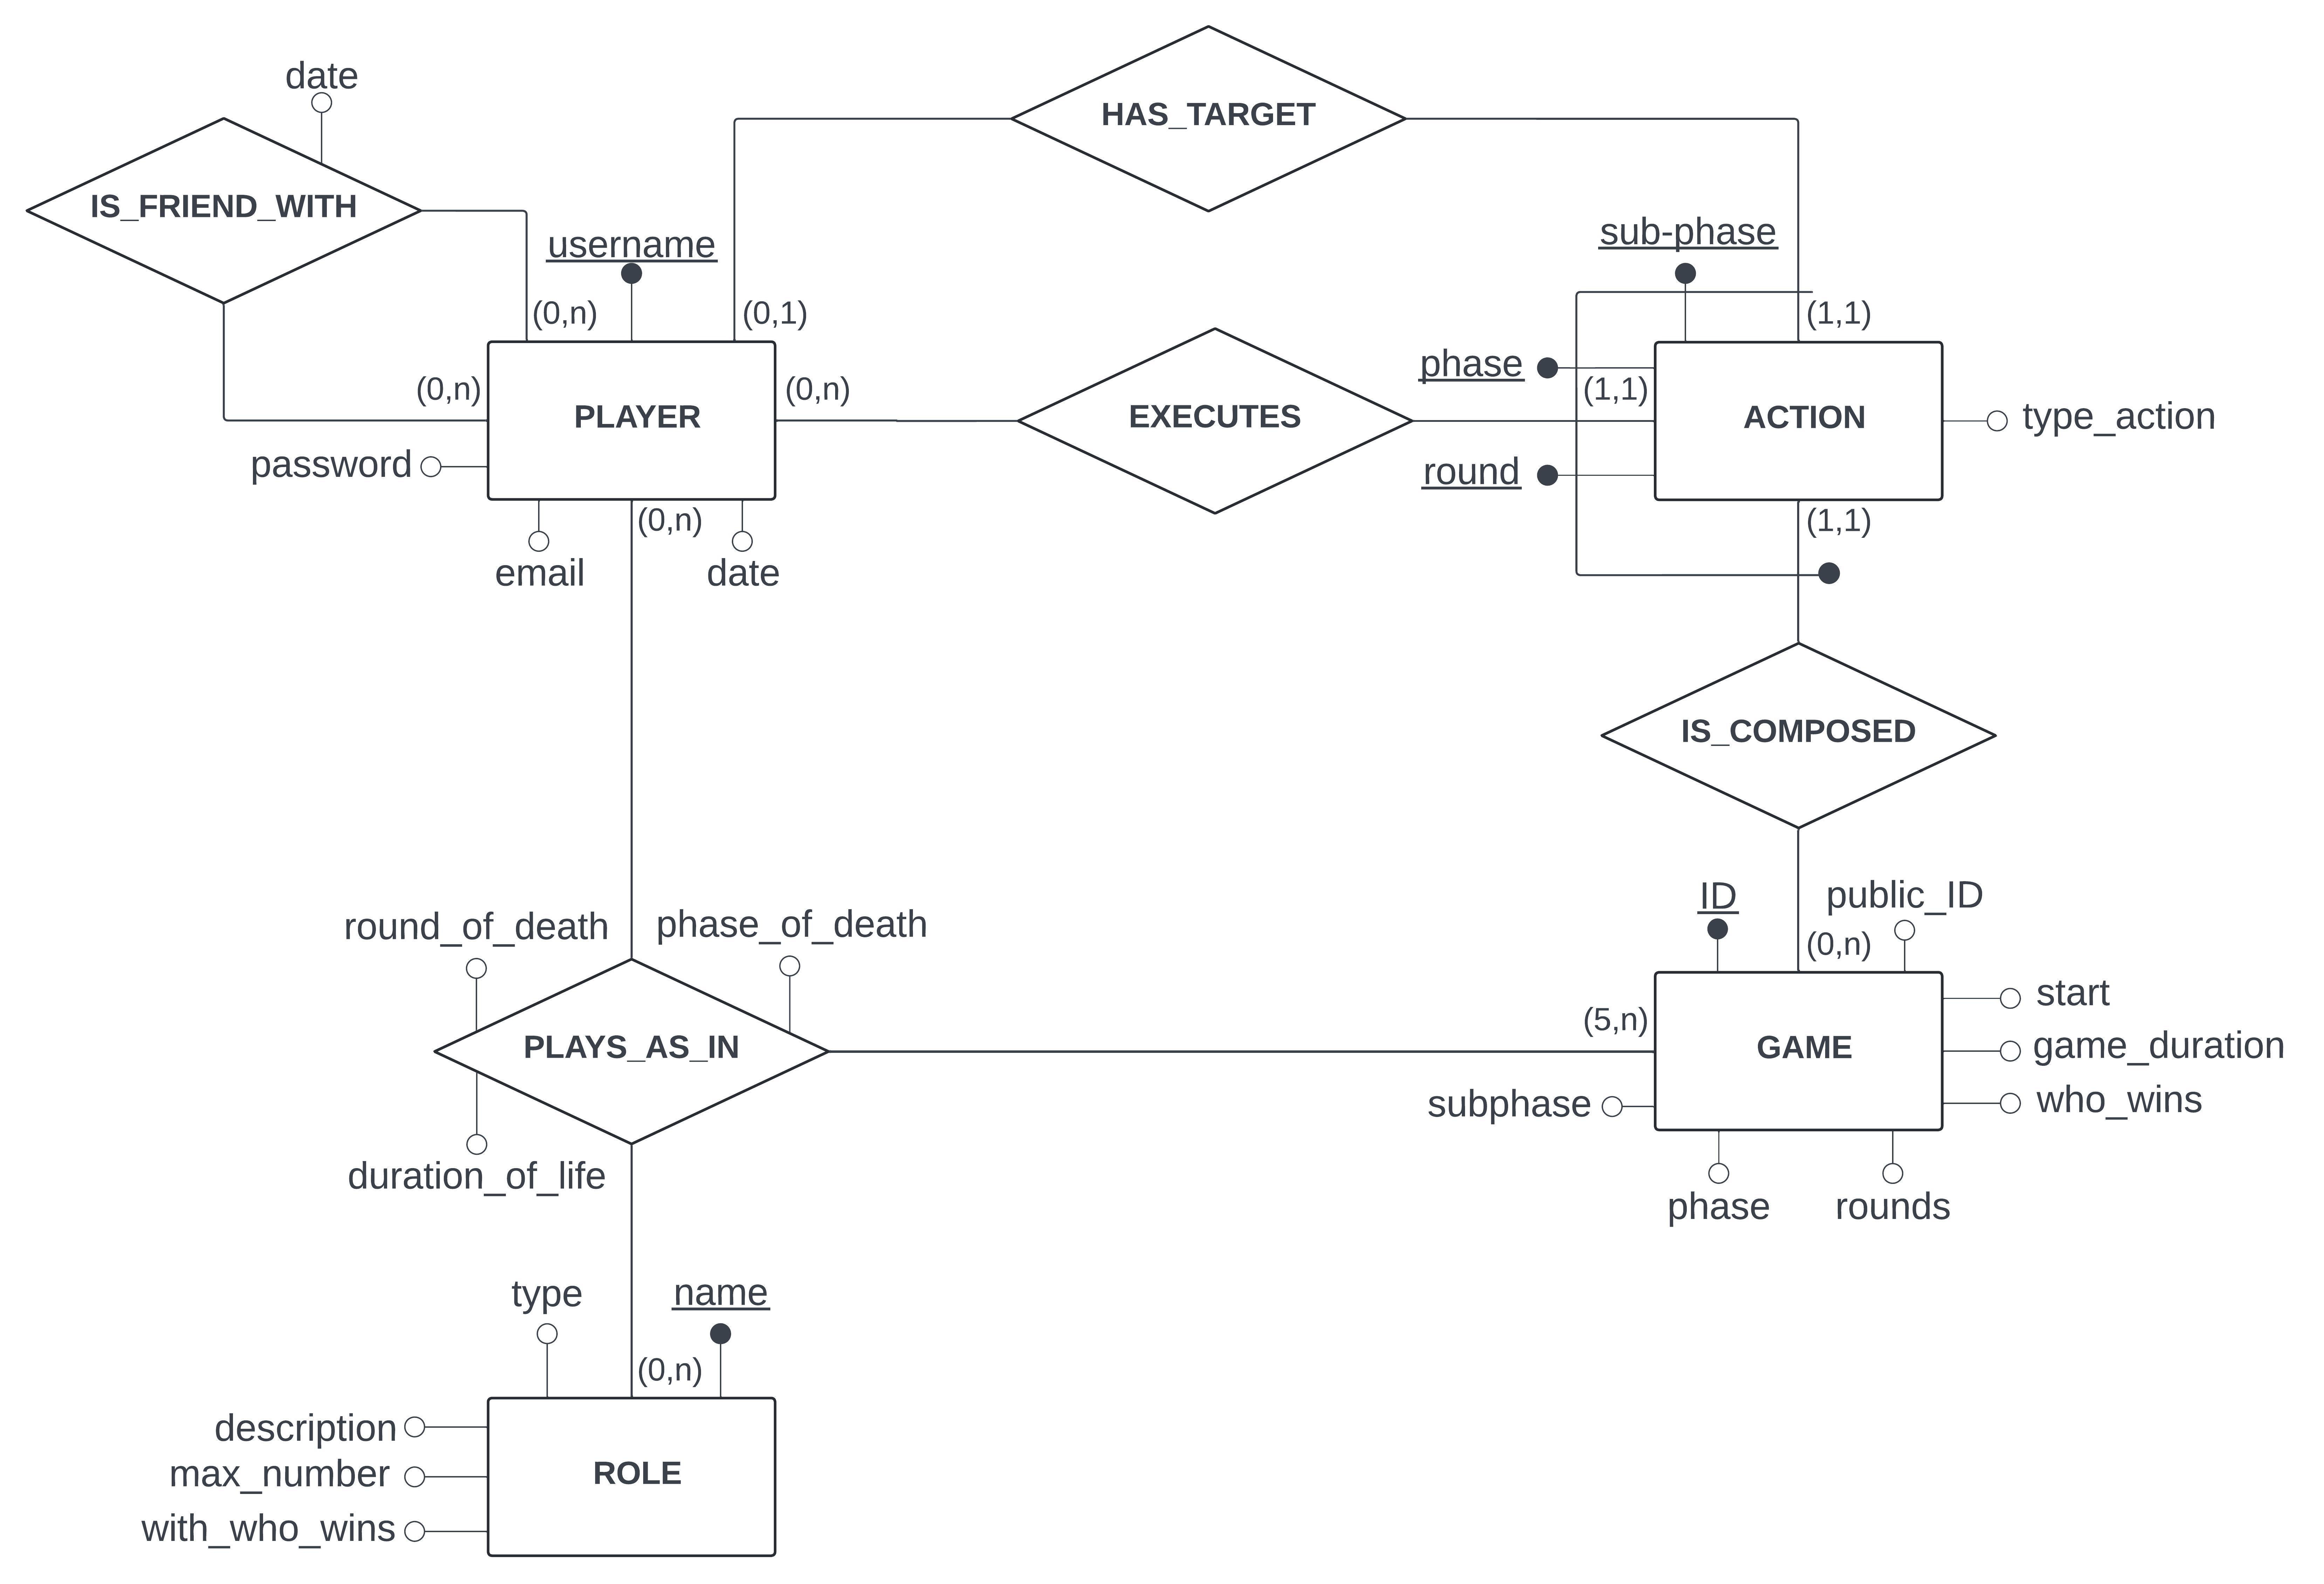
\includegraphics[height=9cm]{images/scheme/er_restructured_f.jpeg}
    \caption{Restructured ER scheme of LUPUS app}
    \label{fig:res_er_scheme}
\end{figure}


\subsubsection{Logical Scheme}
To better visualize the representation of the ER scheme we have created the logic scheme of it. This has permitted to have a better view of the tables that are present in the real database. \\
To create the logic scheme we have done some modifications:
\begin{itemize}
    \item The table ACTION has two "new" attributes one referring to PLAYER (deletion of relation EXECUTES) and one to GAME (deletion of relation IS\_COMPOSED). So the primary key is now composed of fives attributes.
    \item The relation HAS\_TARGET has been added into the table ACTION with a reference to the table PLAYER.
\end{itemize}

The logic scheme of the Lupus App can be seen in the following page [\ref{fig:logic_scheme}].
\begin{figure}[htbp] 
    \centering
    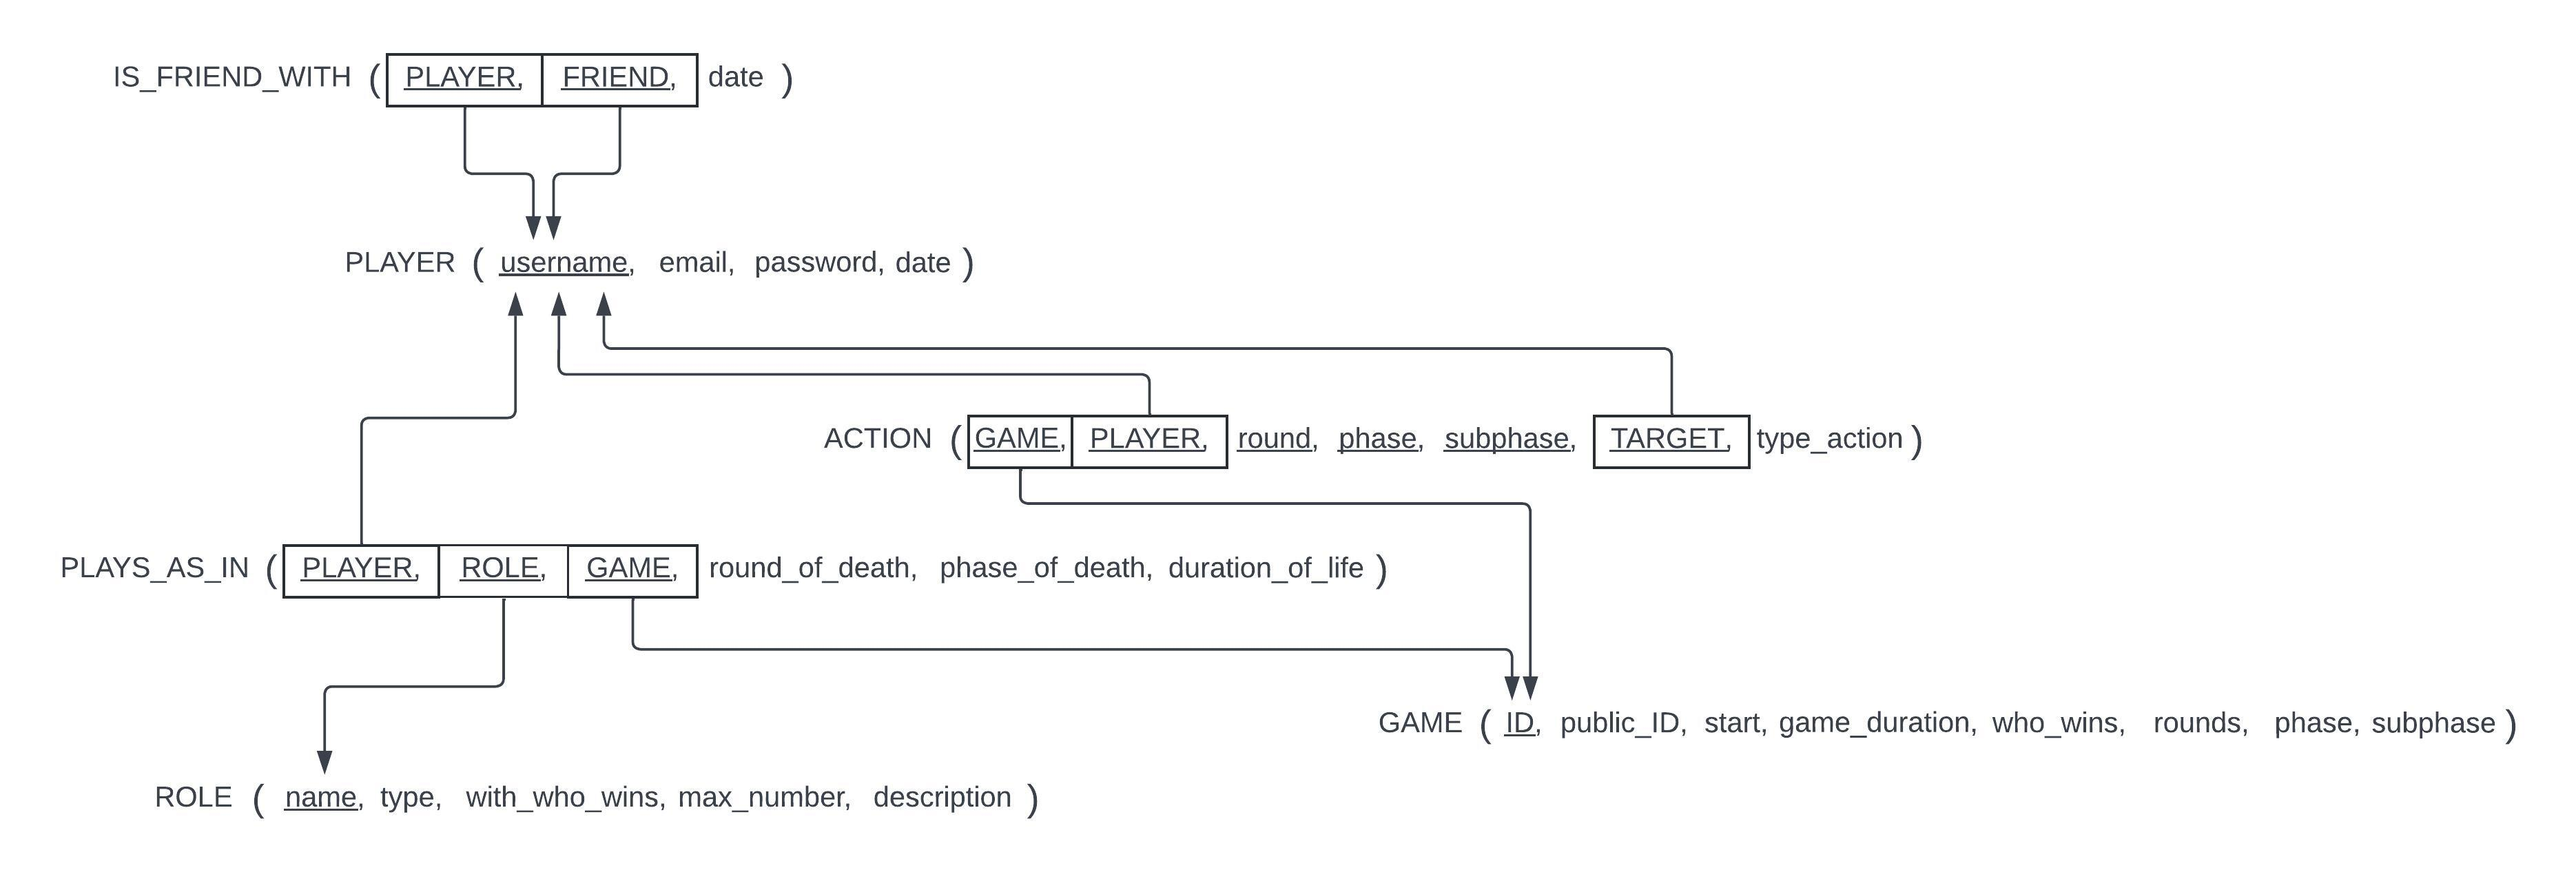
\includegraphics[width=\textwidth, height=5.5cm]{images/scheme/logic_scheme.jpeg}
    \caption{Logic scheme of LUPUS app}
    \label{fig:logic_scheme}
\end{figure}


\subsubsection{Other informations}
The only table in which the insert is not possible is the Role table. In this table there are all the possible roles and, for this reason, insert is not possible. \\
In a future other roles can be implemented, so it can be possible the insert only for developers (maybe the new roles to add will be suggested by players subscribed to the app). \\
The update operation can be done to all the tables except role and action.\\
The delete is only possible in is\_friend\_with tables. This is because a player can decide to delete a friend from his friends list.

\begin{comment}
    \subsubsection{Cose da tenere in considerazione}

. \\


\\

Il voto viene gestito ...
\\


\\
bisogna spiegare cosa vuol dire avere come un ruolo che ruba la vittoria
\\
There is also another attribute description (type: CHARACTER VARYING) that contains useful additional information (can be null).



\end{comment}
